\section{Згорткові нейронні мережі}

Введемо поняття \textbf{маски людини (викладача)}.

Маскою людини \(F^{i}\) будемо називати бінарне прямокутне
зображення \(M^{i}:P \rightarrow \left\{ 0,1 \right\}\), де тим
пікселям, в яких на відповідному кадрі \(F^{i}\) була помічена людина,
відповідає одиниця, а іншим відповідає нуль.


Для локалізації людини були використані так звані \textbf{згорткові нейронні мережі}
(англ. \textit{convolutional neural networks, CNN}).
Це частина машинного навчання, яке називається глибоким навчанням, оскільки використовується
більше двох нейронних шарів разом зі згортковими.

В таких мережах застосовується операція згортки(англ. \textit{convolution})
та пулінгу (англ. \textit{pooling}), батч-нормалізація, та різні функції
активації такі як ReLU, Tanh.

Надалі послідовну комбінацію (згортка + батч-нормалізації + функція активації)
будемо називати згортковим шаром, але кожний автор нейронної мережі
створює свої шари відмінні від вищезазначеного.

\begin{figure}[H]
    \centering
    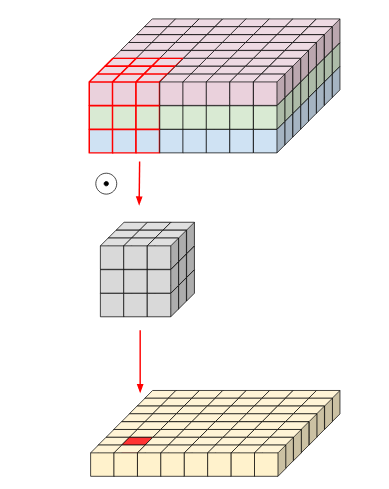
\includegraphics[width=0.3\textwidth]{images/cnn_conv_operation}
    \caption{Ілюстрація взяття звичайної згортки  \cite{deep_wise_sep_conv_website}
        \label{fig:cnn:conv_operation}
    }
\end{figure}

Розглянемо архітектури нейронних мереж, що застосовувались у роботі
для локалізації людини. Всі нищеописані нейронні мережі були використані вже з
натренованими вагами у програмній бібліотеці PyTorch \cite{NEURIPS2019_9015}.
За мету було поставлено підібрати таку мережу, що здатна швидко оброблювати
один знімок навіть на смартфоні. Тому головним критерієм є швидкість.

\subsection{YOLO: You-Only-Look-Once}

YOLO - це сімейство нейронних мереж.

YOLOv1 вперше представили Joseph Redmon.
Вона розв'язує задачу детекції об'єктів як задачу регресії
щодо просторового розділення знайдених областей об'єктів та їх
ймовірностей. Її зараз широко використовують для класифікації та знаходженні об'єктів
оскільки вона здатна оброблювати відео в реальному часі 30 кадрів в секунду
на мобільних пристроях, ща є її найбільшою перевагою серед інших аналогів.

Опишемо коротко головні особливості YOLOv1, оскільки YOLOv5, яка застосовувалась
в роботі є лише модифікацією:
\begin{enumerate}
    \item Спочатку зображення розділяється решіткою $S \times S$.
          Якщо центр об'єкту потрапляє в комірку решітки, тоді ця комірка
          є кандидатом, для подальшої локалізації об'єкта.
    \item Кожна комірка решітки має передбачувати $B$ областей та рівнів
          довіри. Даний рівень довіри показує на скільки модель впевнена,
          що дана комірка містить об'єкт та на скільки точна область.
          Рівень довіри визначається $Pr(Object)*{IOU}_{pred}^{truth}$,
          де $Pr(Object)$- ймовірність об'єкту, ${IOU}_{pred}^{truth}$ - величина
          перетину передбаченої області об'єкту до її справжньої.
          Відповідно якщо модель не знайшла об'єкт цей рівень нульовий.
          Задача, щоб рівень довіри був якомога ближчим до ${IOU}_{pred}^{truth}$.
    \item Кожна область об'єкту складається з 5 чисел: рівень довіри,
          $x, y$ - координати центру об'єкту,  $w, h$ - його ширина та висота.
          Кожна комірка передбачає $C$ умовних ймовірностей $Pr(Class_i|Object)$
\end{enumerate}

\begin{figure}[H]
    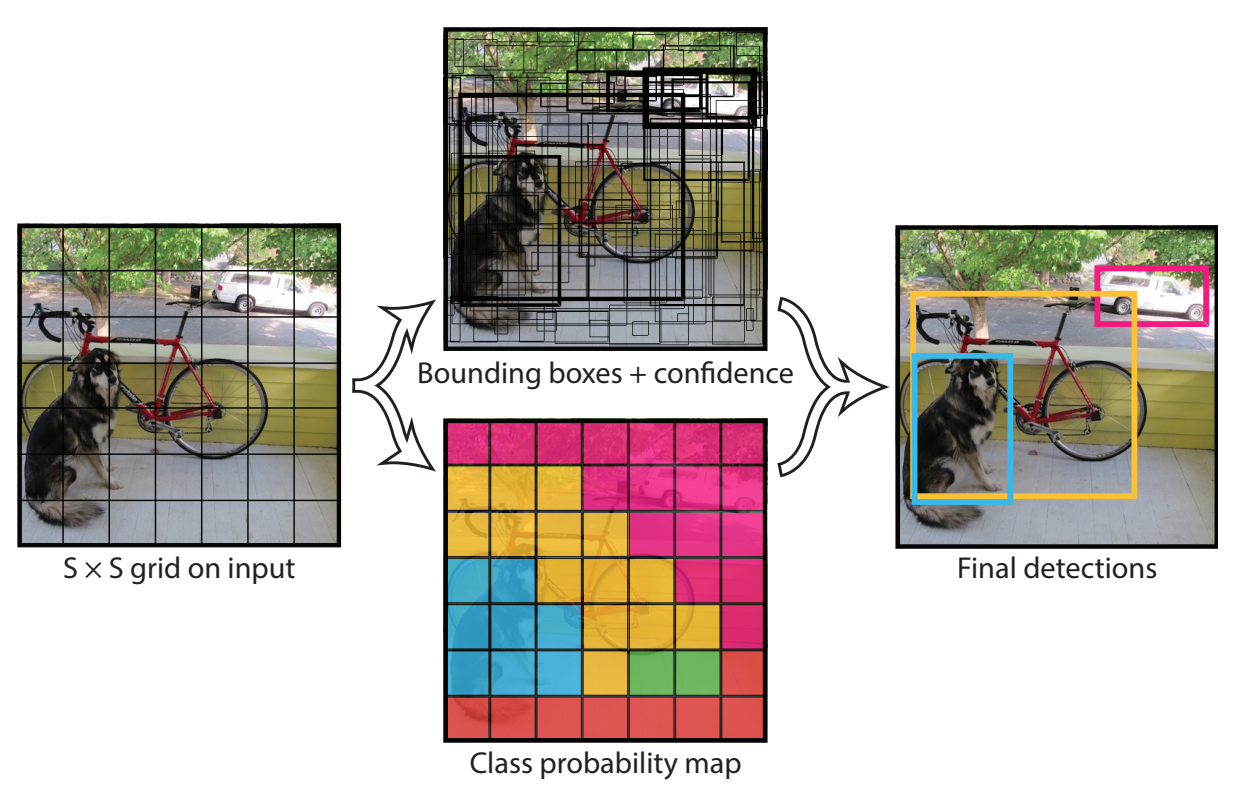
\includegraphics[width=0.5\linewidth]{images/cnn_yolo1}
    \centering
    \caption{Процес локалізації об'єктів мережею YOLO \cite{RedmonYolo}
    }
\end{figure}

Для тренування мережі використовують суму 4 штрафних функцій.

\begin{multline}
    \lambda_{coord}(
    \underbrace{ \sum_{i=0}^{S^2} \sum_{j=0}^{B}
    \mathbb{1}_{ij}^{obj} [(x_i - \widehat{x_i})^2 + (y_i - \widehat{y_i})^2]
    }_\textrm{по координатам центру}\\
    +
    \underbrace{
    \sum_{i=0}^{S^2} \sum_{j=0}^{B}
    \mathbb{1}_{ij}^{obj} [(\sqrt{w_i} - \sqrt{\widehat{w_i}})^2 + (\sqrt{h_i} - \sqrt{\widehat{h_i}})^2]
    }_\textrm{ширини та висоти об'єкту}
    )\\
    +  \underbrace{
        \sum_{i=0}^{S^2} \sum_{j=0}^{B} з
        \mathbb{1}_{ij}^{obj} (C_i - \widehat{C_i})^2
        +
        \lambda_{noobj} \sum_{i=0}^{S^2} \sum_{j=0}^{B} \mathbb{1}_{ij}^{noobj} (C_i - \widehat{C_i})^2
    }_\textrm{точності класифікації}\\
    +  \underbrace{
    \sum_{i=0}^{S^2} \mathbb{1}_{i}^{noobj}\sum_{c \in classes}(p_i(c) -  \widehat{p_i}(c))^2
    }_\textrm{ймовірності класів}
    \label{eq:cnn:yolo_loss}
\end{multline}
, де $\mathbb{1}_{i}^{obj}$ визначає чи знайшовся об'єкт в комірці $i$, а
$\mathbb{1}_{ij}^{obj}$ чи в комірці $i$ в $j$-ій області знаходиться об'єкт.

Загалом архітектура нейронної мережі YOLOv1 складається з 24 згорткових шарів та
2 повнозв'язних лінійних шарів.

\begin{figure}[H]
    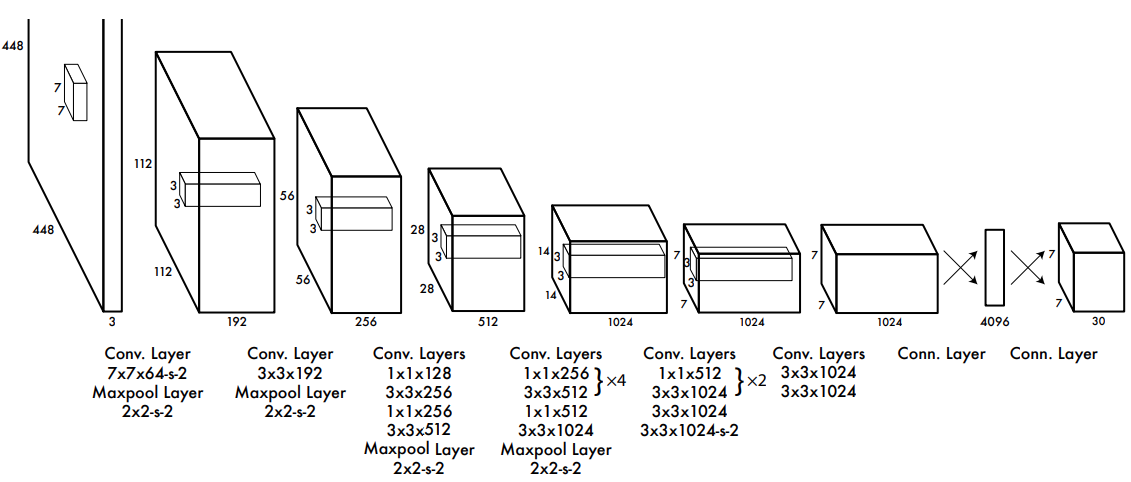
\includegraphics[width=0.8\linewidth]{images/cnn_yolo2}
    \centering
    \caption{Архітектура YOLOv1 \cite{RedmonYolo}
    }
\end{figure}

На момент написання була використана одна з мереж YOLOv5, яка була
розроблена Glenn Jocher вже на програмній бібліотеці PyTorch.

\begin{figure}[H]
    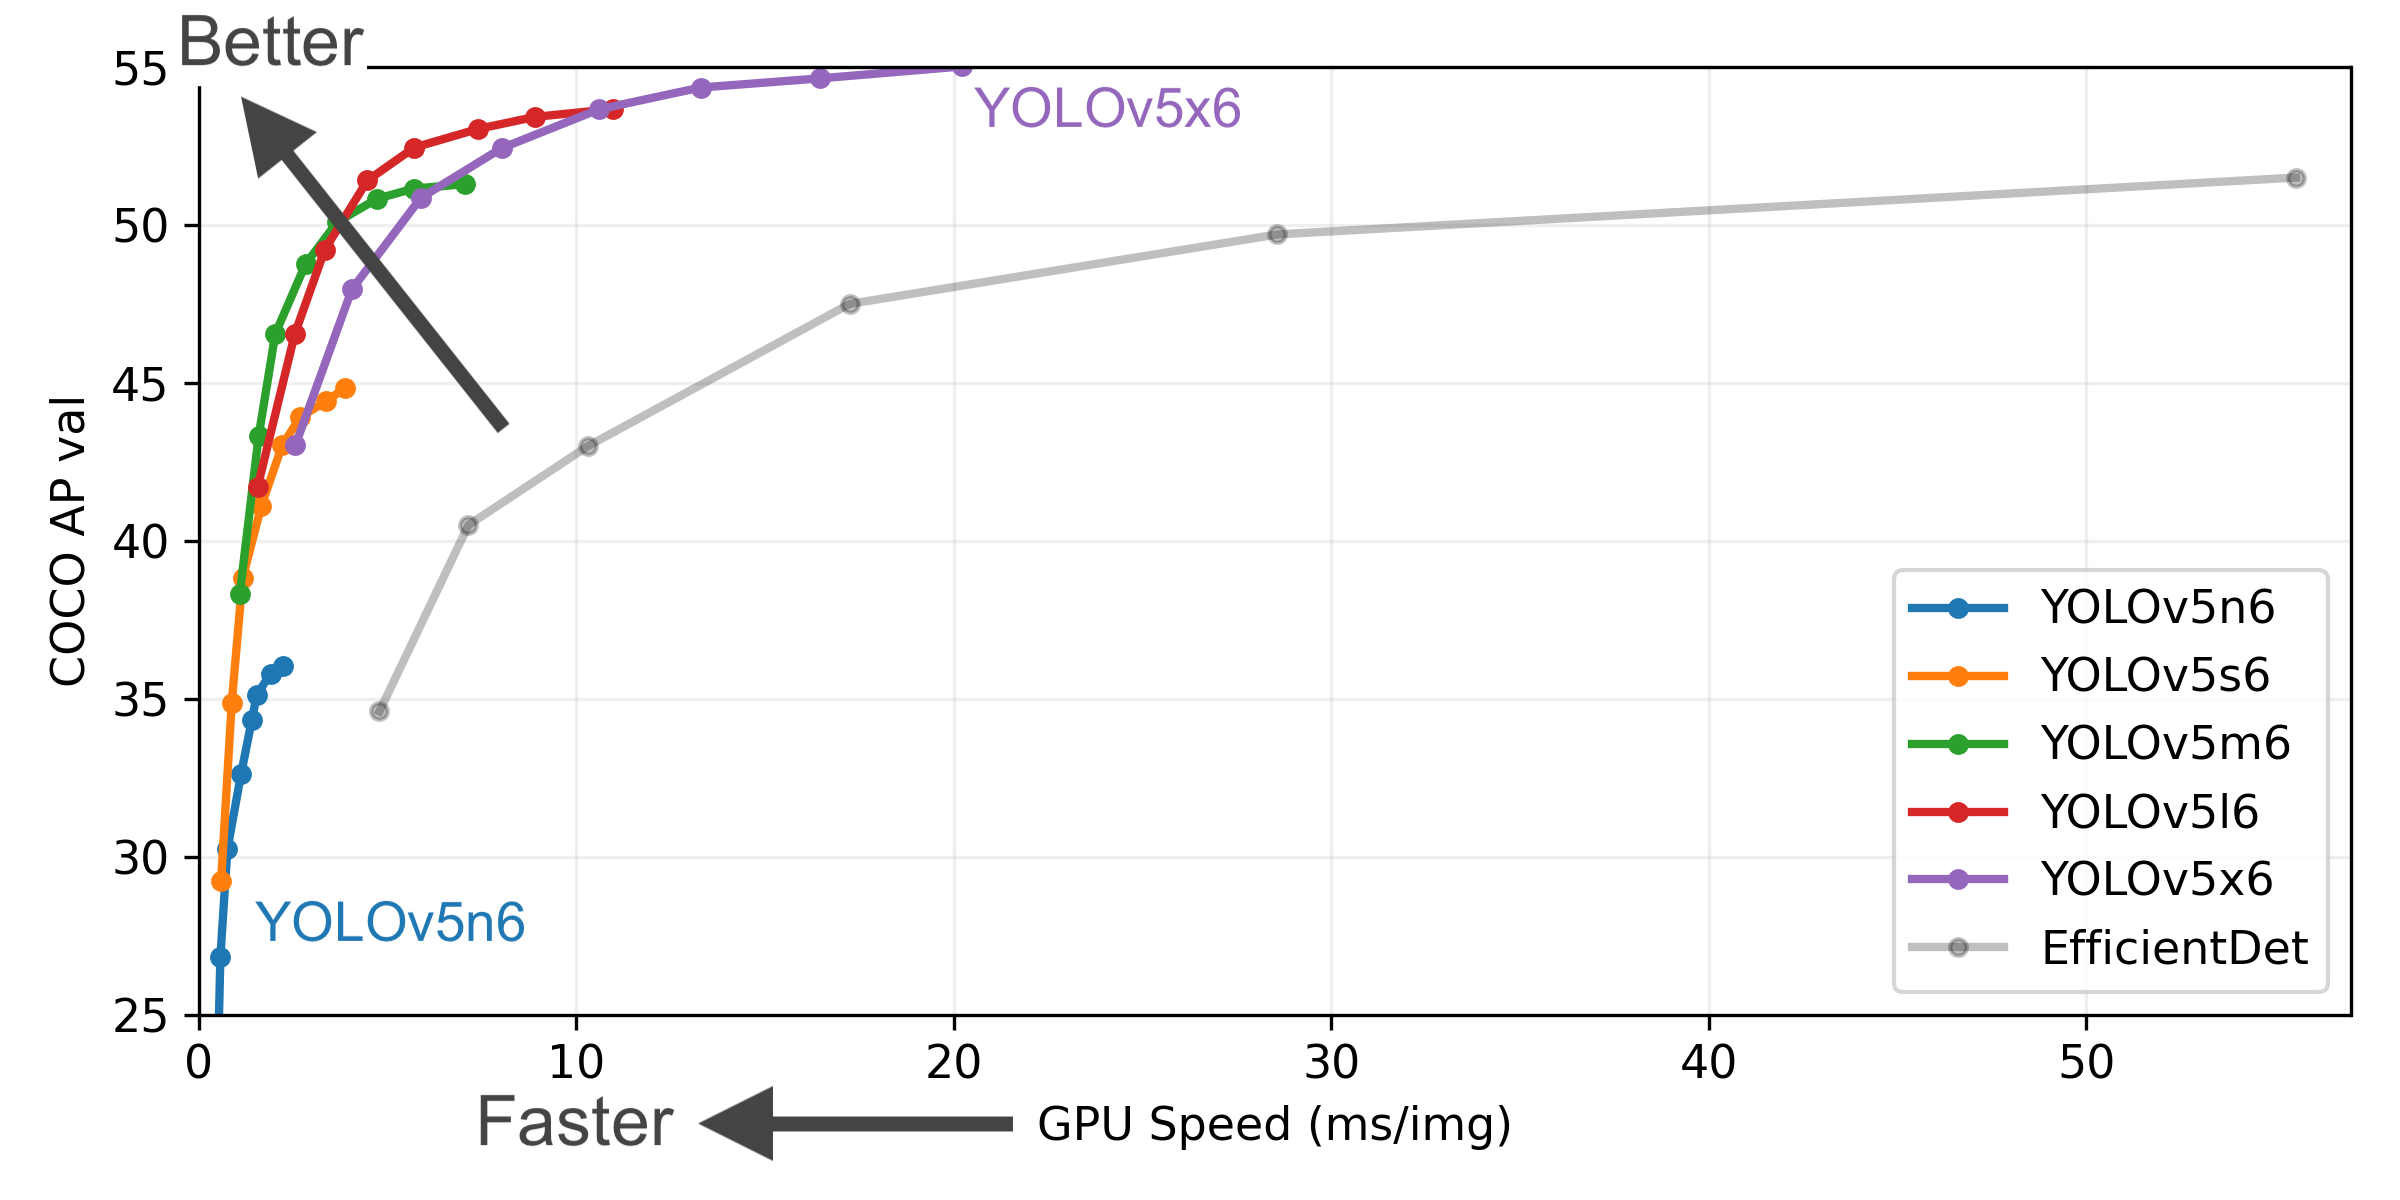
\includegraphics[width=0.5\linewidth]{images/cnn_yolo3}
    \centering
    \caption{Графік залежності точності на датасеті COCO від швидкості обробки однієї
        картинки різними мережами YOLOv5 н
    }
\end{figure}

\subsection{MobileNet}

MobileNet це також ще одне сімейство, що часто використовується у комп'ютерному зорі.
Вперше була представлена у 2017 році науковцями з Google \ref{mobilenetv1}.
Мережі даної категорії теж зробили свою революцію у обчисленні глибоких шарів з
використанням мінімальних обчислювальних ресурсів. Були запропоновані два гіперпараметри,
змінюючи які, можна отримати прирости в швидкості та точності. Мережі MobileNet
застосовуються для локалізації, класифікації об'єктів і також для широкомасштабної
гео-локалізації.

Розглянемо особливості кожної версії MobileNet.

\subsubsection{Mobilenetv1}

Одним з головних задач для побудови першої мережі даного сімейства була заміна
звичайного згорткового шару на новий глибинно просторовий згортковий шар
(англ. \textit{Depth-wise Separable Convolution}).

Нехай маємо:
- квадратне зображення $I$ розмірами $S_I \times S_I \times M$ : широта, висота та
кількість каналів відповідно.
- ядро $C$ розмірами $S_C \times S_C \times M \times N$, де $N$ вихідна розмірність
отриманої згортки.
- вихідна згортка $C$ розмірами $S_K \times S_K \times N$

Тоді формулу звичайної згортки (Рис. \ref{fig:cnn:simple_conv}) можна записати як:

\begin{equation}
    G_{k,l,n} = \sum_{i,j,m} C_{i,j,m,n} · F_{k+i-1, l+j-1,m}
    \label{eq:simple_conv}
\end{equation}

Щоб обчислити дану згортку потрібно $S_C · S_C · M · N · S_I · S_I$ операцій, що
є створює обчислювальні обмеження на мобільний пристрій, якщо наприклад матимемо
декілька таких згорток.
Для вирішення даної проблеми застосовується глибинна згортка (Рис. ). Вона полягає
у отриманні окремої згортки кожного каналу ядра до кожного каналу
зображення.
Нехай $\widehat{C}$ ядро глибинної згортки, тоді маємо:

\begin{equation}
    \widehat{G}_{k,l,n} = \sum_{i,j,m} \widehat{C}_{i,j,m,n} · F_{k+i-1, l+j-1,m}
    \label{eq:deep_wise_conv}
\end{equation}

\begin{figure}[H]
    \centering
    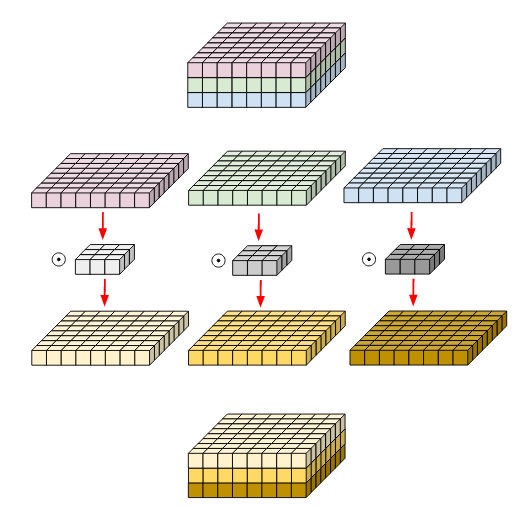
\includegraphics[width=0.35\textwidth]{images/cnn_deep_wise_conv}
    \caption{Ілюстрація взяття глибинної згортки  \cite{deep_wise_sep_conv_website}
        \label{fig:cnn:deep_wise_conv}
    }
\end{figure}

Для обчислення вже цієї згортки треба  $S_C · S_C · M · S_I · S_I$.

Як ми бачимо ми вже позбулись $N$ операцій, але маємо пам'ятати, що
зараз $\widehat{G}$ складається з $M$ окремих вихідних згорток, тому
, щоб створити єдиний вихід додатково до глибинної застосовують ще
й точкову згортку (англ. \textit{point-wise Convolution}), в якій розмір
ядра $1 \times 1$. Тоді маємо
$S_C · S_C · M · S_I · S_I + M · N · S_I · S_I$ операцій.
Дана комбінація має назву глибинно просторова згортка, для
обчислення якої потрібно в $1/N + 1/S_C^2$ менше операцій ніж
для звичайної.

\begin{figure}[H]
    \centering
    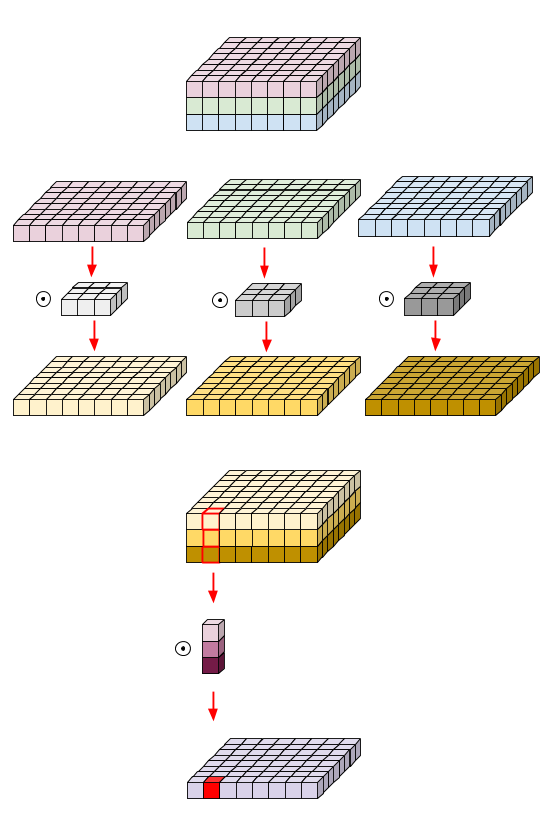
\includegraphics[width=0.35\textwidth]{images/cnn_deep_wise_separable_conv}
    \caption{Ілюстрація взяття глибинно просторової згортки  \cite{deep_wise_sep_conv_website}
        \label{fig:cnn:deep_wise_sep_conv}
    }
\end{figure}


Таке нововведення до глибинного навчання дало змогу в рази пришвидшити
навчання та швидкість нейронної мережі MobileNetv1. Вона використовує
просторово глибинні згортки розміром ядра $3 \times 3$.
Таким чином маємо таку заміну блоку.

\begin{figure}[H]
    \centering
    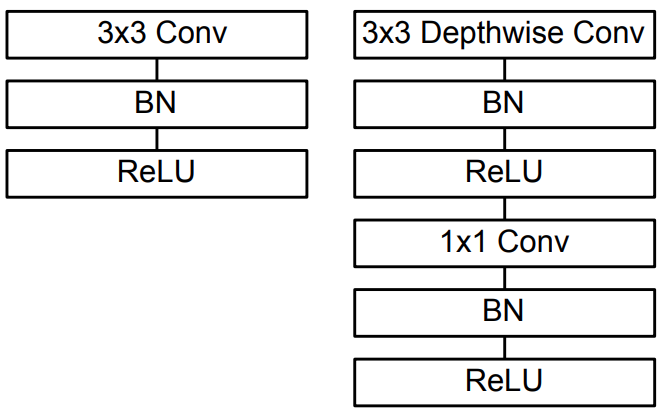
\includegraphics[width=0.4\textwidth]{images/cnn_mobilenetv1_conv_layer}
    \caption{Ліворуч звичайний згортковий шар,
        праворуч згортковий шар у MobileNetv1  \cite{mobilenetv1}
        \label{fig:cnn:mobilenetv1_conv_layer}
    }
\end{figure}

Також варто відмітити ще одну особливість MobileNetv1, а саме два гіперпараметри
ширини та розмірності.
Множник ширини $\alpha$ застосовується, щоб зменшити кожен шар мережі, що
в свою чергу дає приріст у швидкості.
З множником  $\alpha \in (0,1]$ потрібно буде зробити
$S_C · S_C · \alpha M · S_I · S_I + \alpha M · \alpha N · S_I · S_I$ операцій.
Множник розмірності $\rho$ зменшує вхідну картинку і відповідно
розмірність згорток. Разом з $\alpha$  та $\rho \in (0,1]$ необхідно буде
$S_C · S_C · \alpha M · \rho S_I · \rho S_I + \alpha M ·\alpha  N · \rho S_I · \rho S_I$
операцій.

Повна архітектура мережі MobileNetv1 виглядає так:

\begin{figure}[H]
    \centering
    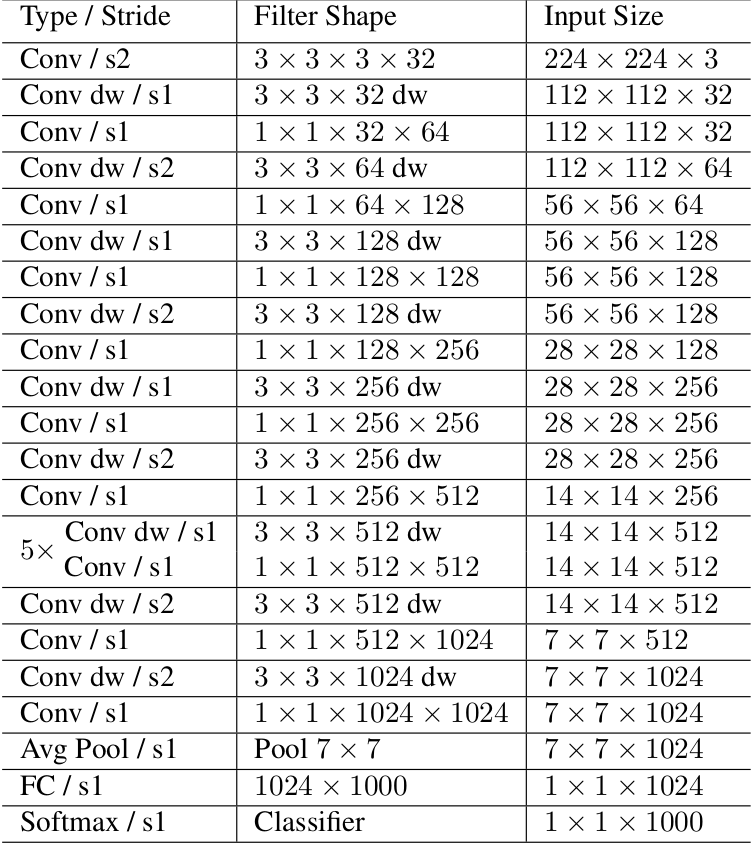
\includegraphics[width=0.4\textwidth]{images/cnn_mobilenetv1_architecture}
    \caption{Архітектура нейронної мережі MobileNetv1   \cite{mobilenetv1}
        \label{fig:cnn:mobilenetv1_architecture}
    }
\end{figure}


\subsubsection{Mobilenetv2}

Вже у 2018 році з'являється 2-га версія мережі MobileNet. Тут автори додали нові зміни в
архітектуру такі як інвертовані залишки (англ. \textit{Inverted Residuals}) та
лінійні вузькі містя (англ.\textit{Linear Bottlenecks}). Також представили застосування
особливостей MobileNetv2 у фреймворку для локалізації SSDLite, що теж був використаний
в даній роботі.

Автори зробили дослідження щодо застосування функції ReLU (rectified linear unit) в
контексті низьких розмірностей. Вводиться поняття \textit{manifold of interest}
різноманітність інтересів - це множина шарів активацій. Була висунута гіпотеза про те що,
різноманітність інтересів з високою розмірністю можна стиснути у підпростір меншої розмірності при
чому зі збереженням інформації.

Розпишемо детальніше з яких кроків складається новий структурний шар:


\begin{enumerate}
    \item Нехай на вході зображення розмірами $S_I · S_I · M$, його приймає перший розширяючий блок.
          Головна особливість цього блоку є новий параметр $t$, що називається розширяючим фактором.
          Найкращими значеннями для нього є $[5,10]$. Менші значення краще застосовувати для меншої мережі,
          а більші відповідно для більших. Саме тут можна побачити різноманітність інтересів.
          Вихід $S_I · S_I · (t·M)$.
    \item Наступним кроком є вже відома глибинна згортка з функцією активації $ReLU6(x) =  min(max(0,x),6)$.
          Вхід $S_I · S_I · (t·M)$, а вихід $(S_I/stride) · (S_I/stride) · (t·M)$, де  $stride$ - шаг згортки.
    \item Далі застосовується точкова згортка, щоб створити єдиний тензор. Як можна побачити на
          Рис. \ref{fig:cnn:mobilenetv2_layer} також застосовуються переваги residual block, де вхід в шар
          поєднується з передостаннім блоком.
\end{enumerate}


\begin{figure}[H]
    \centering
    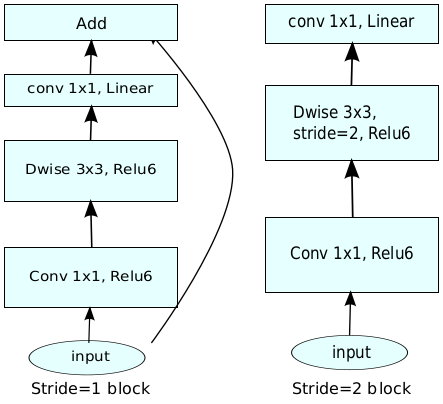
\includegraphics[width=0.5\textwidth]{images/cnn_mobilenetv2_layer}
    \caption{Відмінність MobileNetv2 від MobileNetv1: ліворуч структурний блок MobileNetv2,
        праворуч - MobileNetv1   \cite{mobilenetv2}
        \label{fig:cnn:mobilenetv2_layer}
    }
\end{figure}

\begin{figure}[H]
    \centering
    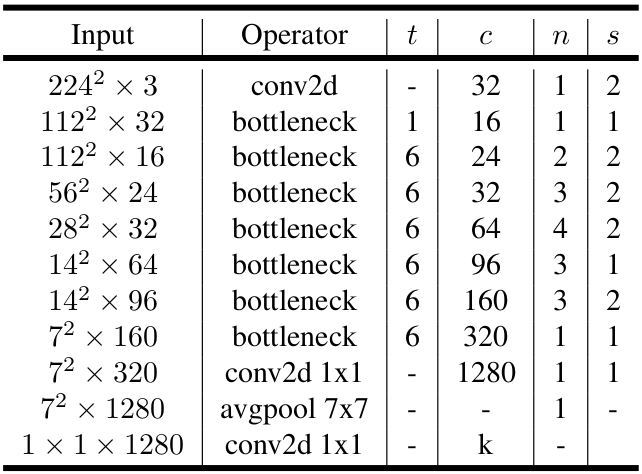
\includegraphics[width=0.5\textwidth]{images/cnn_mobilenetv2_architecture}
    \caption{Архітектура мережі MobileNetv2     \cite{mobilenetv2}
        \label{fig:cnn:mobilenetv2_architecture}
    }
\end{figure}


Також варто відмітити, що автори вдосконалили мережу SSD (Single Shot Detector), він подібний
до YOLO і застосовується для локалізації об'єктів. Автори замінили звичайні згорткові шари
на розширяючі згорткові, які використовуються в MobileNetv2. Таким чином створивши досконалішу
версію SSDLite, про це буде описано пізніше.

\subsubsection{MobileNetv3}

На даний час існує остання 3-тя версія \cite{mobilenetv3} архітектури сімейства нейронні мереж MobileNet.
Тут автори представили вже 2 нейронні мережі MobileNetv3-Small та MobileNetv3-Large.
Це зроблено для того, щоб використовувати модель на слабких і потужних пристроях.
Як запевняють автори MobileNetV3-Small на 6.6 \% точніша за MobileNetv2, а локалізація об'єктів
з MobileNetV3-Large на COCO датасеті на 25 \% швидша при тій же точності.
Головний блок мережі знову змінився у 3-ій версії порівняно з 2-ої.
Окрім того що тут опрацьовуються як ідеї MobileNetv1, MobileNetv2 також автори взяли
до уваги певні особливості мережі MnasNet \cite{mnasnet}, в якій з'явився блок стиснення та збудження
(англ. squeeze and excitation). Мережі з такими блоками називаються Se-Nets.

Мета підходу стиснення та збудження \ref{senet_block} полягає в тому, щоб взяти параметри виходу згортки (нехай
це матриця $u_c$ розмірами $C \times H \times W$) 
як вхід блоку стиснення та збудження,
потім зробити операцію стиснення (маємо $1 \times 1 \times C$), операцію збудження ($1 \times 1 \times C$). Далі
потрібно масштабувати параметри щоб поєднати $u_c$.
Ідея полягає в тому, щоб підвищити чутливість мережі до інформативних ознак і передавати їх
до наступного кроку.

\begin{figure}[H]
    \centering
    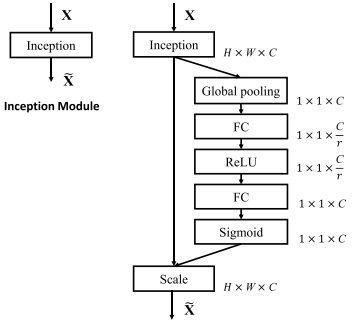
\includegraphics[width=0.5\textwidth]{images/cnn_senet_block}
    \caption{Блок стиснення та збудження      \cite{squeeze_and_excitation_website}
        \label{fig:cnn:senet_block}
    }
\end{figure}

\begin{enumerate}
    \item \textbf{Операція стиснення} полягає у відокремленні глобальної інформації з кожного каналу
          вхідного зображення. Дана операція є краща за звичну згортку, оскільки бере всю інформацію
          з каналу зображення за один раз. Також операція стиснення відома під назвою глобального
          cереднього пулінгу  (англ. global average pooling). Це взяття середнього по кожному каналу.
          \begin{equation}
              z = F_{sq}(u_c) = \frac{\sum_{i=0}^{H} \sum_{j=0}^{W} u_c(i,j)}{H·W}
          \end{equation}
          Вихід $1 \times 1 \times C$.
    \item \textbf{Операція збудження} створює множину ваг для кожного каналу шляхом застосування
          активацій $Sigmoid$ та $ReLU$ для двох повнозв'язних лінійних шарів
          \begin{equation}
              s = F_ex(z,W) = Sigmoid(FC_2ReLu(FC_1z))
          \end{equation}
          Перший лінійний шар $FC_1$ використовується для зменшення розмірності $z$ з деяким
          множником $r$, тому після цього шару розмірність буде $1 \times 1 \times C/r$, а $FC_2$ навпаки
          для збільшення $ReLU(W_1z)$. Знаючи, що значення сигмоїди від 0 до 1, то можна
          масштабувати її вихід із входом в блок $u_c$
          \begin{equation}
              \widetilde{x_c} = F_{scale}(u_c,s_c) = s_c·u_c
          \end{equation}
\end{enumerate}

Автори покращили даний підхід у своїй MobileNetv3, але з використанням
різної нелінійності на кожному шарі. Тут мається на увазі заміна лінійних функцій активацій.
Було вирішено замість нелінійної функції
\begin{equation}
    swish(x) = x·Sigmoid(x)
\end{equation}
використати
\begin{equation}
    h-swish(x) = x·\frac{ReLU6(x + 3)}{6}
\end{equation}
Це пов'язано з тим, що сигмоїда складна в обчисленні
для малопотужних пристроїв.
Також автори помітили, що використання $h-swish(x)$ дає приріст в точності, якщо її
використовувати у глибоких шарах мережі.

Так само як в MnasNet автори MobileNetv3 автори звернулись за допомогою до платформи NAS (neural
architecture structure), яка створена для  підбирання глобальних параметрів мережі.
Тобто NAS рекомендує найкращу знайдену архітектуру, а далі NetAdapt (схожий до NAS) допомагає у підбиранні
параметрів вже всередині одного обчислювального блоку.

Всі вищеописані техніки допомогли створити нову MobileNetv3-Small та MobileNetv3-Large
(Рис. \ref{fig:cnn:mobilenetv3_architecture}).

\begin{figure}[H]
    \centering
    \begin{subfigure}[c]{0.4\textwidth}
        \centering
        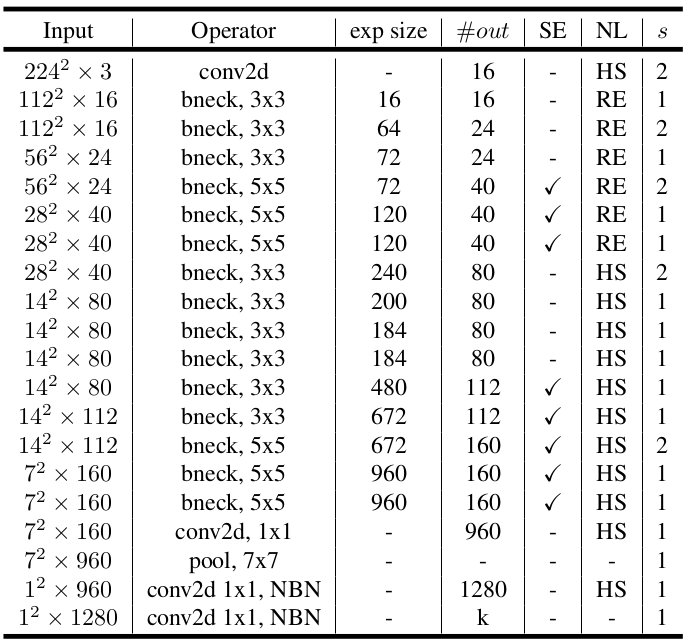
\includegraphics[width=\textwidth]{images/cnn_mobilenetv3_large_architecture}
        \caption{MobileNetv3-Large
        }
    \end{subfigure}
    \begin{subfigure}[c]{0.4\textwidth}
        \centering
        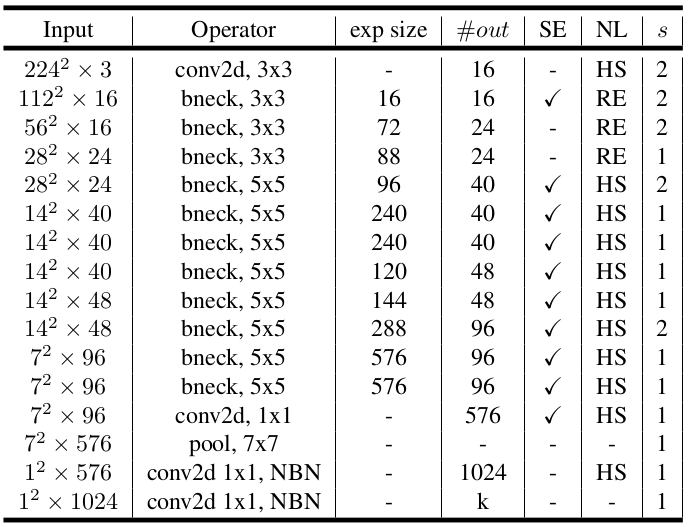
\includegraphics[width=\textwidth]{images/cnn_mobilenetv3_small_architecture}
        \caption{MobileNetv3-Small
        }
    \end{subfigure}
    \caption{Дві архітектури мережі MobileNetv3 \cite{mobilenetv3}
        \label{fig:cnn:mobilenetv3_architecture}
    }
\end{figure}


\subsubsection{SSD: Single Shot Multibox Detector}

Оскільки для відокремлення ознак застосовується в цій роботі SSD із
структурними елементами MobileNetv3, тому є причина показати як саме SSD вдається
локалізовувати об'єкти та його відмінності з YOLO.

Мережа SSD (Рис. \ref{fig:cnn:ssd_architecture}) на відміну від YOLO проганяє зображення
через шари лише один раз. Це пояснюється словами в назві Single Shot. SSD
використовує задачу MultiBox регресії
локалізованих областей. Розпишемо її детальніше.

\begin{figure}[H]
    \centering
    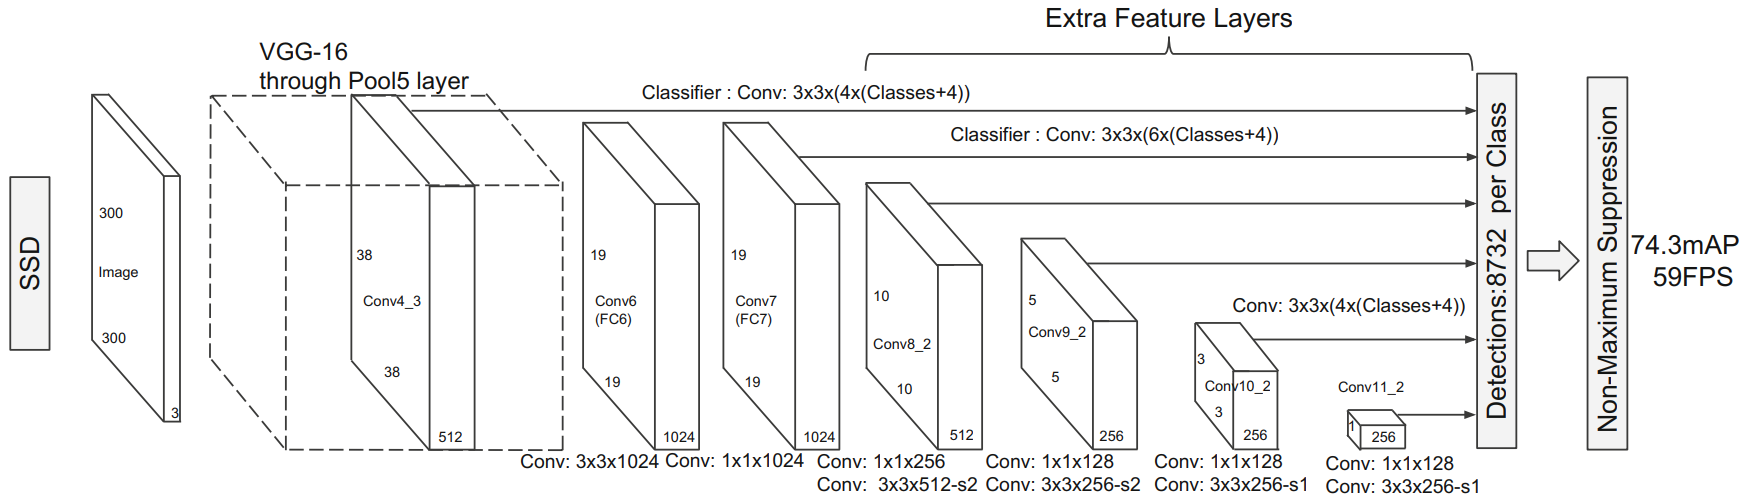
\includegraphics[width=0.8\textwidth]{images/cnn_ssd_architecture}
    \caption{Архітектура мережі SSD на основі VGG-16    \cite{ssd}
        \label{fig:cnn:ssd_architecture}
    }
\end{figure}

Головна задача MultiBox це оцінювати як точно локалізувати об'єкти. Тут використовується
дві штрафні функції: довіри, що основана на категоріальній перехресній ентропії та
локалізації з L2 нормою, яка показує як точно справжня область об'єкту співпадає
із передбаченою.

Варто також помітити, що SSD застосовує вже фіксовані області для подальшого передбачення
із згортками малого ядра.
Чим більше фіксованих областей, то тим більша точність локалізації об'єкту,
але тим довша обробка фото.

Принцип відокремлення інформативних ознак SSD полягає у розбитті зображення на решітку
(Рис. \ref{fig:cnn:ssd_work_example}) (аналогічно YOLO). Запускається класифікатор
і вирішує чи брати ту чи іншу клітинку
кандидатом на локалізацію. Для кожної фіксованої області обчислюється розмір
області та рівень довіри для кожної категорії об'єктів.

\begin{figure}[H]
    \centering
    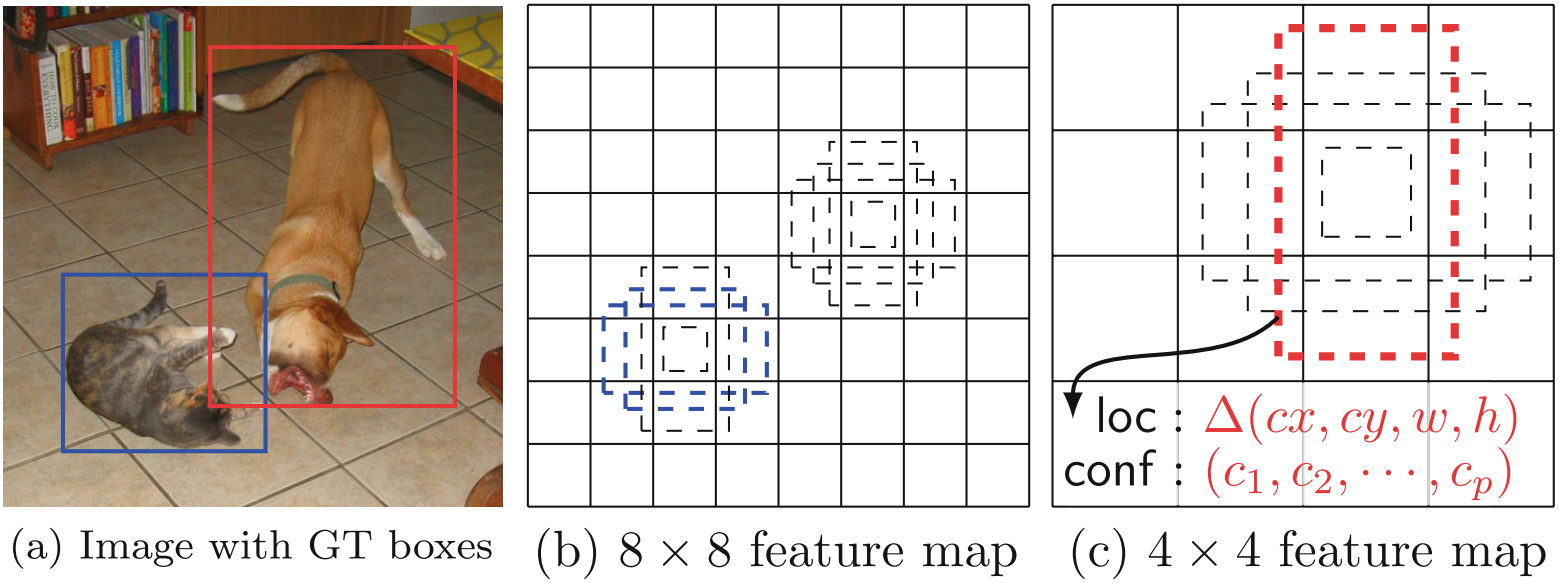
\includegraphics[width=0.7\textwidth]{images/cnn_ssd_work_example}
    \caption{Приклад роботи SSD для локалізації об'єктів \cite{ssd}
        \label{fig:cnn:ssd_work_example}
    }
\end{figure}


\subsubsection{Faster R-CNN}

Говорячи про детекцію і класифікацію об'єктів не можна не згадати про також відомий
клас згорткових нейронних мереж як R-CNN (region-based convolutional neural network).

Перша мережа R-CNN складалась з 3 незалежних один від одного етапів.
На першому генерується 2000 пропозицій областей за допомогою
вибіркового пошуку. Далі ці області проходять стиснення розміру до якогось
фіксованого. Останній етап це метод опорних векторів вже з натренованими 
вагами, який і робить класифікацію.

R-CNN не була досить потужною, оскільки використовувала вибірковий пошук, 
який займає чимало часу. Також варто відмітити, що потрібно зберігати чимало
кешованих даних для натренованої мережі, щоб натренувати CNN.

Багато проблем було вирішено вже з новою Fast R-CNN. В ній відсутні етапи як такі,
а вся архітектура складається з одного модуля, що в рази полегшує
навчання мережі. Тут також вводиться новий шар ROI Pooling, головна ціль якого 
надати вектори ознак фіксованої довжини. Даний шар розбиває кожний запропонований 
регіон на решітку, в кожній клітинці якій потім знаходиться максимальне значення
(операція max pooling). Але навіть якщо і  Fast R-CNN швидша за R-CNN в ній досі 
лишився вибірковий алгоритм.

У Faster R-CNN \cite{faster_rcnn}, який саме теж тестувався для локалізації людини в
цій роботі, запропоновано використовувати RPN (Region Proposal Network), як спосіб 
генерації областей-кандидатів та Fast R-CNN для виявлення об'єктів в цих областях.
Ці два етапи поєднуються в одну мережу за допомогою поширення ознак (feature sharing).


\textbf{RPN}  приймає на вхід картинку, і повертає множину координат прямокутних областей як подальших
кандидатів для класифікації з їхніми мірами присутності об'єкту. RPN - повнозв'язна 
згорткова мережа, що значить в ній немає лінійних шарів. Саме вона стала заміною
вибіркового алгоритму у Fast R-CNN. 

\begin{figure}[H]
    \centering
    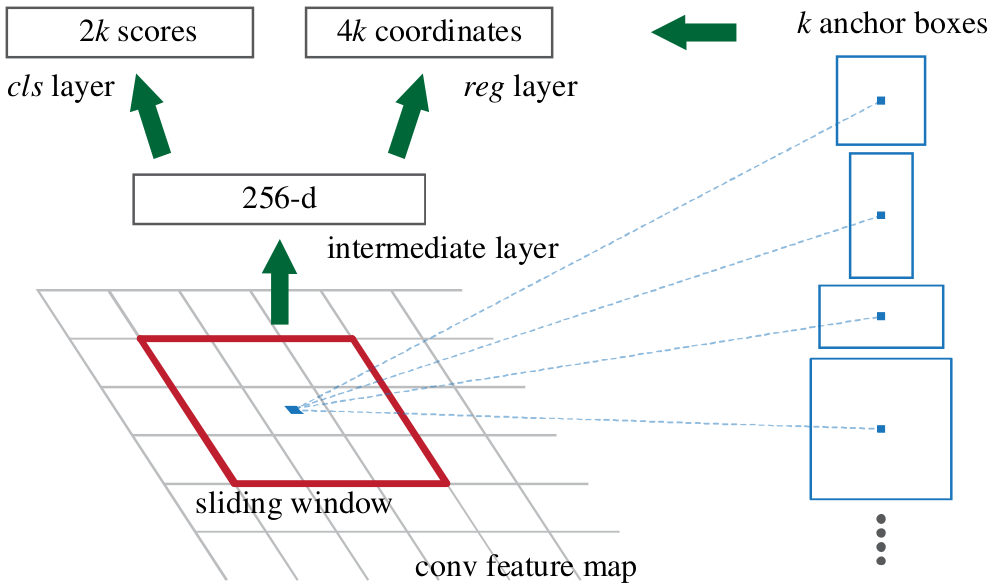
\includegraphics[width=0.5\textwidth]{images/cnn_faster_rcnn_rpn}
    \caption{Архітектура мережі RPN \cite{faster_rcnn}
        \label{fig:cnn:faster_rcnn_rpn}
    }
\end{figure}

У RPN ми застосовуємо принцип ковзкого вікна (sliding window) на згортковій мапі ознак,
отриманої після останнього згорткового шару. Кожне таке вікно відображається 
на вектор меншої розмірності. Для кожного вікна генеруються прямокутні області-кандидати, 
що називаються якірними регіонами (anchor boxes) з параметрами масштабу та співвідношення сторін.
Далі цей вектор подається на вхід двом повнозв'язним
шарам: локалізації об'єктів(box-regression layer) та класифікації(box-classification layer).
Використання якірних регіонів дозволяє детектувати об'єкти практично будь-якого масштабу та 
пов'язувати ознаки RPN з Fast R-CNN.

Як вже було сказано, принцип поширення ознак дозволяє поєднати вихід RPN як вхід в Fast R-CNN.
Головна його ідея у використанні одних і тих же згорток у двох мережах, що дозволяє тренувати 
RPN разом  з Fast R-CNN,  а не окремо.

\begin{figure}[H]
    \centering
    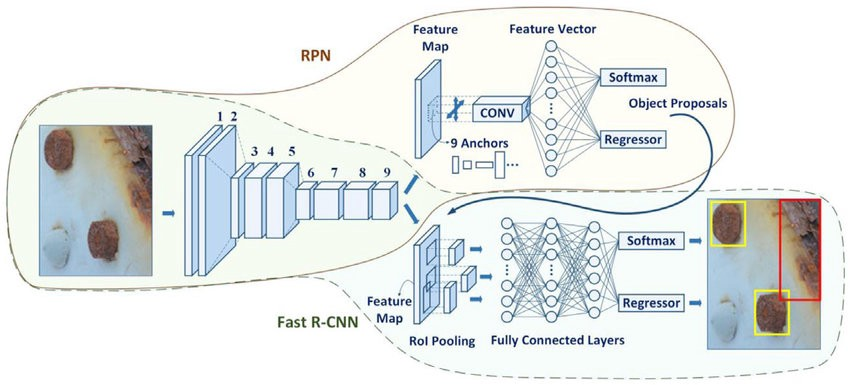
\includegraphics[width=0.7\textwidth]{images/cnn_faster_rcnn_architecture}
    \caption{Архітектура мережі Faster R-CNN \cite{faster_rcnn_website}
        \label{fig:cnn:faster_rcnn_architecture}
    }
\end{figure}


\clearpage